%% BioMed_Central_Tex_Template_v1.06
%%                                      %
%  bmc_article.tex            ver: 1.06 %
%                                       %

%%IMPORTANT: do not delete the first line of this template
%%It must be present to enable the BMC Submission system to
%%recognise this template!!

%%%%%%%%%%%%%%%%%%%%%%%%%%%%%%%%%%%%%%%%%
%%                                     %%
%%  LaTeX template for BioMed Central  %%
%%     journal article submissions     %%
%%                                     %%
%%          <8 June 2012>              %%
%%                                     %%
%%                                     %%
%%%%%%%%%%%%%%%%%%%%%%%%%%%%%%%%%%%%%%%%%


%%%%%%%%%%%%%%%%%%%%%%%%%%%%%%%%%%%%%%%%%%%%%%%%%%%%%%%%%%%%%%%%%%%%%
%%                                                                 %%
%% For instructions on how to fill out this Tex template           %%
%% document please refer to Readme.html and the instructions for   %%
%% authors page on the biomed central website                      %%
%% http://www.biomedcentral.com/info/authors/                      %%
%%                                                                 %%
%% Please do not use \input{...} to include other tex files.       %%
%% Submit your LaTeX manuscript as one .tex document.              %%
%%                                                                 %%
%% All additional Figures and files should be attached             %%
%% separately and not embedded in the \TeX\ document itself.       %%
%%                                                                 %%
%% BioMed Central currently use the MikTex distribution of         %%
%% TeX for Windows) of TeX and LaTeX.  This is available from      %%
%% http://www.miktex.org                                           %%
%%                                                                 %%
%%%%%%%%%%%%%%%%%%%%%%%%%%%%%%%%%%%%%%%%%%%%%%%%%%%%%%%%%%%%%%%%%%%%%

%%% additional documentclass options:
%  [doublespacing]
%  [linenumbers]   - put the line numbers on margins

%%% loading packages, author definitions

% \documentclass[twocolumn]{bmcart}% uncomment this for twocolumn layout and comment line below
% \documentclass[linenumbers, doublespacing]{bmcart}
\documentclass{bmcart}
% \bibliographystyle{unsrtnat}

%%% Load packages
\usepackage{amsthm,amsmath}
\RequirePackage{natbib}
% \RequirePackage[authoryear]{natbib}% uncomment this for author-year bibliography
\RequirePackage{hyperref}
% \usepackage[utf8]{inputenc} %unicode support
% \usepackage[applemac]{inputenc} %applemac support if unicode package fails
% \usepackage[latin1]{inputenc} %UNIX support if unicode package fails
\usepackage{lmodern}% http://ctan.org/pkg/lm
\usepackage{subcaption} %for subfigures
\usepackage{graphicx} %graphics support to specify path
\usepackage{csvsimple} %insert tables using .csv files
\usepackage{caption}
\usepackage{adjustbox}

%%%%%%%%%%%%%%%%%%%%%%%%%%%%%%%%%%%%%%%%%%%%%%%%%
%%                                             %%
%%  If you wish to display your graphics for   %%
%%  your own use using includegraphic or       %%
%%  includegraphics, then comment out the      %%
%%  following two lines of code.               %%
%%  NB: These line *must* be included when     %%
%%  submitting to BMC.                         %%
%%  All Figure files must be submitted as      %%
%%  separate graphics through the BMC          %%
%%  submission process, not included in the    %%
%%  submitted article.                         %%
%%                                             %%
%%%%%%%%%%%%%%%%%%%%%%%%%%%%%%%%%%%%%%%%%%%%%%%%%


% \def\includegraphic{}
% \def\includegraphics{}
\bibliographystyle{unsrt}

\graphicspath {{figures/}}

%%% Put your definitions there:
\startlocaldefs

% ignore command 
\newcommand{\ignore}[2]{\hspace{0in}#2}

\endlocaldefs


%%% Begin ...
\begin{document}

%%% Start of article front matter
\begin{frontmatter}

\begin{fmbox}
\dochead{Methodology}

%%%%%%%%%%%%%%%%%%%%%%%%%%%%%%%%%%%%%%%%%%%%%%
%%                                          %%
%% Enter the title of your article here     %%
%%                                          %%
%%%%%%%%%%%%%%%%%%%%%%%%%%%%%%%%%%%%%%%%%%%%%%

\title{Tissue Enrichment Analysis (TEA)}

%%%%%%%%%%%%%%%%%%%%%%%%%%%%%%%%%%%%%%%%%%%%%%
%%                                          %%
%% Enter the authors here                   %%
%%                                          %%
%% Specify information, if available,       %%
%% in the form:                             %%
%%   <key>={<id1>,<id2>}                    %%
%%   <key>=                                 %%
%% Comment or delete the keys which are     %%
%% not used. Repeat \author command as much %%
%% as required.                             %%
%%                                          %%
%%%%%%%%%%%%%%%%%%%%%%%%%%%%%%%%%%%%%%%%%%%%%%

\author[
   addressref={aff1},                   % id's of addresses, e.g. {aff1,aff2}
   % email={dangeles@caltech.edu}   % email address
]{\inits{DA}\fnm{David} \snm{Angeles-Albores}}
\author[
   addressref={aff1},                   % id's of addresses, e.g. {aff1,aff2}
   % email={raymond@caltech.edu}   % email address
]{\inits{RYL}\fnm{Raymond YN} \snm{Lee}}
\author[
   addressref={aff1},                   % id's of addresses, e.g. {aff1,aff2}
   % email={azurebrd@caltech.edu}   % email address
]{\inits{JC}\fnm{Juancarlos} \snm{Chan}}
\author[
   addressref={aff1},
   corref={aff1},
   email={pws@caltech.edu}
]{\inits{PWS}\fnm{Paul W} \snm{Sternberg}}


%%%%%%%%%%%%%%%%%%%%%%%%%%%%%%%%%%%%%%%%%%%%%%
%%                                          %%
%% Enter the authors' addresses here        %%
%%                                          %%
%% Repeat \address commands as much as      %%
%% required.                                %%
%%                                          %%
%%%%%%%%%%%%%%%%%%%%%%%%%%%%%%%%%%%%%%%%%%%%%%

\address[id=aff1]{%                           % unique id
  \orgname{HHMI and California Institute of Technology, Division of Biology and Biological Engineering}, % university, etc
  \street{1200 E California Blvd},                     %
  \postcode{91125},                               % post or zip code
  \city{Pasadena},                              % city
  \cny{USA}                                    % country
}



%%%%%%%%%%%%%%%%%%%%%%%%%%%%%%%%%%%%%%%%%%%%%%
%%                                          %%
%% Enter short notes here                   %%
%%                                          %%
%% Short notes will be after addresses      %%
%% on first page.                           %%
%%                                          %%
%%%%%%%%%%%%%%%%%%%%%%%%%%%%%%%%%%%%%%%%%%%%%%


\end{fmbox}% comment this for two column layout

%%%%%%%%%%%%%%%%%%%%%%%%%%%%%%%%%%%%%%%%%%%%%%
%%                                          %%
%% The Abstract begins here                 %%
%%                                          %%
%% Please refer to the Instructions for     %%
%% authors on http://www.biomedcentral.com  %%
%% and include the section headings         %%
%% accordingly for your article type.       %%
%%                                          %%
%%%%%%%%%%%%%%%%%%%%%%%%%%%%%%%%%%%%%%%%%%%%%%

\begin{abstractbox}

\begin{abstract} % abstract
\parttitle{Background} %if any
Over the last ten years, there has been explosive development in tools
for measuring gene expression. These tools can identify thousands of altered 
genes between conditions, but understanding these datasets and forming hypotheses based on them remains challenging. One way to analyze these datasets is to associate ontologies (hierarchical, descriptive vocabularies
with controlled relations between terms) with genes and to look for enrichment of specific terms. Although gene ontology (GO) is available for   \emph{Caenorhabditis~elegans}, it does not include anatomical information.
\parttitle{Results} %if any 
We have developed a tool for identifying  enrichment of \emph{C.~elegans} tissues among gene sets and generated a website GUI where users can access this tool. Since a common drawback to ontology enrichment analyses is result verbosity, we developed a very simple trimming algorithm to reduce the ontology size by an order of magnitude. We adjusted these filters and validated our tool using a set of 30  gold standards from Expression Cluster data in WormBase and we show our tool can even discriminate between embryonic and larval tissues and can even identify tissues down to the single-cell level. We used our tool to identify multiple neuronal tissues that are down-regulated due to pathogen infection in \emph{C.~elegans}.
\parttitle{Conclusions} %if any
Our Tissue Enrichment Analysis (TEA) can be found at \url{www.wormbase.org/tea}, and can be downloaded using Python's standard pip installer. It tests a slimmed-down \emph{C.~elegans} tissue ontology for enrichment of specific terms and provides users with a  text and graphic representation of the results. 
\end{abstract}

%%%%%%%%%%%%%%%%%%%%%%%%%%%%%%%%%%%%%%%%%%%%%%
%%                                          %%
%% The keywords begin here                  %%
%%                                          %%
%% Put each keyword in separate \kwd{}.     %%
%%                                          %%
%%%%%%%%%%%%%%%%%%%%%%%%%%%%%%%%%%%%%%%%%%%%%%

\begin{keyword}
\kwd{Gene Ontology}
\kwd{Anatomy Ontology}
\kwd{WormBase}
\kwd{RNA-seq}
\kwd{High-throughput biology}
\end{keyword}

% MSC classifications codes, if any
%\begin{keyword}[class=AMS]
%\kwd[Primary ]{}
%\kwd{}
%\kwd[; secondary ]{}
%\end{keyword}

\end{abstractbox}
%
%\end{fmbox}% uncomment this for twcolumn layout

\end{frontmatter}

%%%%%%%%%%%%%%%%%%%%%%%%%%%%%%%%%%%%%%%%%%%%%%
%%                                          %%
%% The Main Body begins here                %%
%%                                          %%
%% Please refer to the instructions for     %%
%% authors on:                              %%
%% http://www.biomedcentral.com/info/authors%%
%% and include the section headings         %%
%% accordingly for your article type.       %%
%%                                          %%
%% See the Results and Discussion section   %%
%% for details on how to create sub-sections%%
%%                                          %%
%% use  \cite{...} to cite references        %%
%%   \cite{koon} and                         %%
%%   \cite{oreg,khar,zvai,xjon,schn,pond}    %%
%%  \nocite{smith,marg,hunn,advi,koha,mouse}%%
%%                                          %%
%%%%%%%%%%%%%%%%%%%%%%%%%%%%%%%%%%%%%%%%%%%%%%

%%%%%%%%%%%%%%%%%%%%%%%%% start of article main body
% <put your article body there>

%%%%%%%%%%%%%%%%
%% Background %%
%%
\section*{Background}
	RNA-seq and other high-throughput methods in biology have the ability to identify thousands of genes that are altered between conditions. These genes are often correlated in their biological characteristics or functions, but identifying these functions remains challenging. To interpret these long lists of genes, biologists need to abstract genes into concepts that are biologically relevant to form hypotheses about what is happening in the system. One such abstraction method relies on Gene Ontology (GO). GO provides a controlled set of hierarchically ordered terms~\cite{TheGeneOntologyConsortium2000a, TheGeneOntologyConsortium2015} that provide detailed descriptions about the molecular, cellular or biochemical functions of any gene. For a given gene list, existing software programs can query whether a particular term is enriched~\cite{Mi2009, McLean2010, Huang2009}. One area of biological significance that GO does not include is anatomy. One way to address this shortcoming is to use a `tissue ontology' that provides a complete anatomical description for an organism (e.g `tissue', `organ' or `specific cell'), in this case for \emph{C.~elegans}~\cite{Lee2003}. Cells and tissues are physiologically relevant units with broad, relatively well-understood functionalities amenable to hypothesis formation. The \emph{C.~elegans} database, WormBase~\cite{Howe2016}, maintains a curated list of gene expression data from the literature. Here we provide a new framework that analyzes a user-input list for enrichment of specific cells and tissues. %As such, we believe that identification of tissues is likely to provide researchers with enough information to be able to form hypotheses about the physiological responses of an organism to a specified condition.

Another problem frequently associated with GO enrichment analysis is that it is often difficult to interpret due to the large number of terms associated with a given gene. %There exist a number of GO analytic tools for use by the community but a shared complaint for many programs is the very large number of GO terms that are significantly associated with any given gene list.
DAVID, a common tool for GO enrichment analysis, clusters enriched terms into broad categories~\cite{Huang2007}, whereas PANTHER~\cite{Mi2009, Mi2013} attempts to solve this issue by employing a manually reduced ontology, GOslim (pers. comm., H. Yu and P. Thomas). To reduce verbosity, we have filtered our ontology using a small set of well-defined criteria to remove terms that do not contribute additional information. To our knowledge, such filtering has not been performed in an algorithmic fashion for a biological ontology before---indeed, DAVID does not employ term trimming \emph{a priori} of testing, but rather fuzzy clustering \emph{post} testing to reduce the number of ontology terms. Other pruning tools do exist (see for example~\cite{Kim2007}), but the pruning is query-dependent. We believe our trimming methodology strikes a good balance between detailed tissue calling and conservative testing.

%Our tool is available within WormBase and provides users with a text-based file of the enrichment results as well as a simple and clear graph of the results that exhibit the largest fold-change enrichment.

\section*{Results}
\subsection*{Generating a Gene-Tissue Dictionary}
\subsubsection*{Reducing term redundancy through a similarity metric}
As a first step to generate our tissue enrichment software, we wished to select tissue terms that were reasonably well-annotated, yet specific enough to provide insight and not redundant with other terms. %We also wanted to avoid testing tissues at levels where annotation redundancy becomes problematic. For example, several left and right neurons have at least 25 annotated genes and we may want to include them for enrichment testing. 
For example, nematodes have a number of neurons that are placed symmetrically along the left/right body axis, and are functionally similar. These left/right neuronal pairs (which are sisters in the ontology) have almost identical annotations, with at most one or two gene differences between them%. We reasoned that when two tissues have almost identical annotations
, and therefore we cannot have statistical confidence in differentiating between them. As a result, testing these sister tissues provides no additional information compared with testing only the parent node to these sisters. %We refer to such sisters as `redundant'. 
To identify redundancy, we defined a similarity metric (see \emph{Methods} section and Figure~\ref{fig:simdiagram}) that can be used to identify sisters that have very high similarity between them; alternatively, redundant sisters could be identified if a single sister had a very high similarity score. We referred to these two scoring criteria as `avg' and `any' respectively.

\subsubsection*{Terminal branch terms and parent terms can be
safely removed in an algorithmic fashion }
Another problem arises from the ontology being scarcely populated. Many nodes have 0-10 annotations, which we consider too few to accurately test. To solve this issue, we implemented a straightforward trimming strategy. For a given terminal node, we test whether the node has more than a threshold number of annotations. If it does not, the node is removed. The next higher node in the branch is tested and removed recursively until a node which satisfies the condition is found. At that point, no more nodes can be removed from that branch. This is guaranteed by the structure of the ontology: parent nodes inherit all of the annotations of all of their descendants, so the number of annotated terms monotonically increases with increasing term hierarchy (see Figure~\ref{fig:trim_ends}). In this way, we ensure that our term dictionary includes only those tissues that are considered sufficiently well annotated for statistical purposes.

Additionally, we reasoned that, for any parent node, if all its daughters were selected for testing, there was no additional benefit to test the parent. %In other words, if all the daughter nodes are tested, there is little additional information to be gained by including the parent node. To address this issue 
We removed parent nodes from the analysis if all their daughter nodes passed the annotation threshold (see Figure~\ref{fig:trim_roots}). We called this a ceiling filter. Applying these three filters reduced the number of ontology terms by an order of magnitude. 

%Finally, we also wanted to remove as many terms as possible from the dictionary with the goals of reducing covariance between terms and decreasing multiple testing. Decreasing covariance between terms is important because we employ a frequentist approach that assumes all terms are independent. Covariation  between terms means that if one of these tissues tests significant, the other terms are much more likely to pass significance testing as well. This makes adequate correction for false positive rates considerably more difficult.

\subsubsection*{Filtering greatly reduces the number of nodes used for analysis}
By itself, each of these filters can reduce the number of nodes employed for analysis, but applying the filters in different orders removes different numbers of nodes (not all the filters are commutative). We chose to always execute annotation and similarity thresholding first, followed by the ceiling filter.
%If the ceiling filter is applied before any other filter, only terminal nodes will remain, since all the parents have complete daughter sets. Since terminal nodes are the most poorly annotated, after applying the remaining filters very few nodes will be left behind if any. On the other hand, applying the ceiling operator after trimming and redundancy filtering will result in greater numbers of nodes. We always applied the ceiling at the end. 
For validation (see below) we made a number of different dictionaries. The original ontology has almost 6,000 terms of which 1675 have at least 5 gene annotations. After filtering, dictionary sizes ranged from 21 to a maximum of 460 terms, which shows the number of terms in a scarcely annotated ontology can be reduced by an order of magnitude through the application of a few simple filters (see Table~\ref{tab:DictionarySpecs}). These filters were used to compile a static dictionary that we employ for all analyses (see \emph{Validation of the algorithm and parameter selection} section for details). 

\subsection*{Tissue enrichment testing via a hypergeometric model}
Having built a static dictionary, we generated a Python script that implements a significance testing algorithm based on the hypergeometric model. Briefly, the hypergeometric model tests the probability of observing $n_i$ occurences of a tissue $i$ in a list of size $M$ if there are $m_i$ labels for that tissue in a dictionary of total size $N$ that are drawn without replacement. Mathematically, this is expressed as: 

\begin{eqnarray}\label{hypergeometric}
	\mathrm{P}(n_i | N, m_i, M) = \frac{\dbinom{m_i}{n_i} \dbinom{M-m_i}{N - n_i}}{\dbinom{N}{n_i}}\text{.}
\end{eqnarray}

Although a user will input gene IDs, we test the number of ocurrences of a term within the gene list, so a single gene can contribute to multiple terms. Due to the discrete nature of the hypergeometric distribution, this algorithm can generate artifacts when the list is small. To avoid spurious results, a tissue is never considered significant if there are no annotations for it in the user-provided list.

Once the p-values for each term have been calculated, we apply a standard FDR correction using a Benjamini-Hochberg step-up algorithm~\cite{Benjamini1995}. FDR corrected p-values are called q-values. Genes that have a q-value less than a given alpha are considered significant. Our default setting is an alpha of 0.1. 

Users input a gene list using any valid gene name for \emph{C.~elegans}. These names are processed into standard WormBase gene IDs (WBGene IDs). The program returns a table containing all the enriched terms and associated  information such as number of terms in gene list and expected number of terms.%with significant tissues, their associated q-value, the expected number of hits for a list of that size, the observed number of hits and the enrichment fold change ($\text{observed hits} /\text{expected hits}$)
 Finally, the program can also return a bar chart of the enrichment fold change for the fifteen tissues with the lowest measured q-values. The bars in the graph are sorted in ascending order of q-value and then in descending order of fold-change. Bars are colored for ease of viewing, and color does not convey information. Our software is implemented in an easy to use GUI (see Figure~\ref{fig:GUIresults}). Anatomy terms are displayed in human-readable format followed by their unique ontology ID (WBbt ID). In summary, each time the ontology annotations are updated, a new trimmed ontology is generated using our filters; in parallel, users can submit their gene lists through WormBase for testing, with results output in a number of formats (see Figure~\ref{fig:workflow}).

\subsection*{Validation of the algorithm and optimizing parameter selection}
We wanted to select a dictionary that included enough terms to be specific beyond the most basic %largest -> basic
 \emph{C.~elegans} tissues, yet would minimize the number of spurious results and which had a good dynamic range in terms of enrichment fold-change. Larger tissues are correlated with better annotation, so increasing term specificity is associated with losses in statistical power.
%The phrase below doesn't seem useful
%To our knowledge there is no good method for assessing false-positive or false-negative results for annotations.
% Gold-standard data sets were annotated gene lists derived from the corresponding Expression Cluster data available in the WS252 version of WormBase.
To help us select an appropriate dictionary and validate our tool, we used a set of 30 gold standards based on microarray and RNA-seq literature which are believed to be enriched in specific tissues~\cite{Gaudet2004a, Spencer2011, Cinar2005, Watson2008a, Pauli2006, Portman2004, Fox2007, Smith2010}. These data sets are annotated gene lists derived from the corresponding Expression Cluster data in WormBase. Some of these studies have been used to annotate gene expression, and so they did not constitute an independent testing set. To correct this flaw, we built a clean dictionary that specifically excluded all annotation evidence that came from these studies.

As a first attempt to select a dictionary, we generated all possible combinations of dictionaries with minimal annotations of 10, 25, 33, 50 and 100 genes and similarity cutoffs of 0.9, 0.95 and 1, using `avg' or `any' similarity thresholding methods (see Table~\ref{tab:DictionarySpecs}). The number of remaining ontology terms was inversely correlated to the minimum annotation cutoff, and was largely insensitive to the similarity threshold in the range we explored. Next, we analyzed all 30 datasets using each dictionary. Because of the large number of results, instead of analyzing each set of terms individually, we measured the average q-value for significantly enriched terms in each dataset without regard for the perceived accuracy of the terms that tested significant. We found that the similarity threshold mattered relatively little for any dictionary. We also noticed that the `any' thresholding method resulted in tighter histograms with a mode closer to 0. For this reason, we chose the `any' method for dictionary generation. The average q-value increased with decreasing annotation cut-off (see Figure~\ref{fig:qvals}), which reflects the decreasing statistical power associated with fewer annotations per term, but we remained agnostic as to how significant is the trade-off between power and term specificity. Based on these observations, we ruled out the dictionary with the 100 gene annotation cut-off: it had the fewest terms and its q-values were not low enough in our opinion to compensate for the trade-off in specificity. 

%dictionaries that work well
To select between dictionaries generated between 50, 33 and 25 annotation cut-offs, and also to ensure the terms that are selected as enriched by our algorithm are reasonable, we looked in detail at the enrichment analysis results.
%Work well
% TODO add WBbt codes!
Most results were comparable and expected. For some sets, all dictionaries performed well. For example, in our `all neuron enriched sets'~\cite{Spencer2011, Watson2008a} all terms were neuron-related %including mechanosensory neurons, thermosensitive neurons, interneurons, ganglions and male rays 
regardless of the dictionary used (see Table~\ref{tab:interagree}). On the other hand, for a set enriched for germline precursor expression in the embryo~\cite{Spencer2011}, the 50 cutoff dictionary was only able to identify `oocyte WBbt:006797' which is not a germline precursor, although it is germline related; whereas the two smaller dictionaries singled out actual germline precursor cells---at the 33 cutoff, our tool identified the larval germline precursor cells `Z2' and `Z3' as enriched, and at the 25 gene cutoff the embryonic germline precursor terms `P$_4$',`P$_3$' and `P$_2$' were identified in addition to `Z2' and `Z3'. 
%Differences between dictionaries
We also queried an intestine precursor set~\cite{Spencer2011}. Notably, this gene set yielded no enrichment when using the 25 cutoff dictionary, nor when using the 50 cutoff dictionary. However, the 33 cutoff dictionary identified the E lineage, which is the intestinal precursor lineage in \emph{C.~elegans}, as enriched. Both of these results capture specific aspects of \emph{C.~elegans} that are well known to developmental biologists. 

%Bad stuff.
Not all queries worked equally well. For example, a number of intestinal  sets~\cite{Spencer2011, Pauli2006} were not enriched in intestine-related terms in any dictionary, but were enriched for pharynx and hypodermis. We were  surprised that intestinal gene sets performed poorly, since the intestine is a relatively well-annotated tissue. 

%Dictionary intra-agreement
We assessed the internal agreement of our tool by using independent gene sets that we expected to be enriched in the same tissues. We used two  pan-neuronal sets~\cite{Spencer2011, Watson2008a}; two PVD sets~\cite{Spencer2011, Smith2010}; and two  GABAergic sets~\cite{Spencer2011, Cinar2005}.%; two  pharyngeal gene sets~\cite{Spencer2011, Gaudet2004a}; and two  intestinal gene sets~\cite{Spencer2011, Pauli2006}. 
Overall, the tool has good internal agreement. On most sets, the same terms were enriched, although order was somewhat variable (see Table~\ref{tab:interagree}), and most high-scoring terms were preserved between sets. %The intestinal gene-sets and pharyngeal gene sets comparisons were exceptions, since at least one gene set showed no enriched terms in all dictionaries, so we did not consider them as informative for assessing internal agreement. 
All comparisons can be found online in our Github repository (see Availability of data and materials). Overall, the dictionary generated by a 33 gene annotation cutoff with 0.95 redundancy threshold using the `any' criterion performed best, with a good balance between specificity, verbosity and accuracy, so we selected this parameter set to generate our static dictionary. As of this publication, the testable dictionary contains 261 terms. 


\subsection*{Applying the tool}
We applied our tool to the RNA-seq datasets developed by Engelmann et al.~\cite{Engelmann2011} to gain further understanding of their underlying biology. Engelmann et al. exposed young adult worms to 5 different pathogenic bacteria or fungi for 24 hours, after which mRNA was extracted from the worms for sequencing. We ran TEA on the genes Engelmann \emph{et al} identified as up- or down-regulated. Initially we noticed that genes that are down-regulated tend to be twice better annotated on average than genes that were up-regulated, suggesting that our understanding of the worm immune system is scarce, in spite of important advances made over the last decade. Up-regulated tissues, when detected, almost always included the hypodermis and excretory duct. Three out of the five samples showed enrichment of neuronal tissues or neuronal precursor tissues amongst the down-regulated genes. As an independent verification, we also performed GO analysis using PANTHER on the down-regulated genes for \emph{D.~coniospora}. These results also showed enrichment in terms associated with neurons (see Figure~\ref{fig:Dcon}). A possible explanation for this neuronal association might be that the infected worms are sick and the neurons are beginning to shut down; an alternative hypothesis would be that the worm is down-regulating specific neuronal pathways as a behavioral response against the pathogen. Indeed, several studies~\cite{Meisel2014, Zhang2005} have provided evidence that \emph{C.~elegans} uses chemosensory neurons to identify pathogens. %One bacterium did not ellicit the same pattern of down-regulation of neuronal-associated genes. \emph{E.~faecalis} showed increased expression of genes associated with neuronal tissues, hinting that \emph{E.~faecalis} may have a different pathogenic profile. 
Our results highlight the involvement of various \emph{C.~elegans} neuronal tissues in pathogen defense.

\section*{Discussion}
%TEA Discussion
We have presented a tissue enrichment analysis tool that employs a standard hypergeometric model to test the \emph{C.~elegans} tissue ontology. We use a hypergeometric function to test a user-provided gene list for enrichment of anatomical terms in \emph{C.~elegans}. Our hope is that the physiological relevance of anatomical terms will enable researchers to make hypotheses about high-dimensionality data. Specifically, we believe an enriched term may broadly suggest one of two hypotheses: if a list is enriched in a particular anatomical region, that anatomical region is affected by the experimental treatment; alternatively, the anatomical regions that are enriched reflect biologically relevant interactions between tissues. We believe the first hypothesis is a reasonable hypothesis to make in the case of whole-worm RNA-seq data for example, whereas the second hypothesis may be more plausible in cases where a researcher already knows what tissues a particular gene list came from, as may be the case in single-cell RNA-seq. 

%Other tools
Our tool relies on an annotation dictionary that is continuously updated primarily with data from single gene qualitative analyses, does not require retraining and does not require ranked genes. To our knowledge, this is the first tool that tests tissue enrichment  in \emph{C.~elegans} via the hypergeometric method, but similar projects exist for humans and zebrafish~\cite{Lee2013, Prykhozhij2013}, highlighting the relevance of our tool for high-dimensionality biology. Chikina \emph{et al}~\cite{Chikina2009} have previously reported a tissue enrichment model for \emph{C.~elegans }based on a Support Vector Machine classifier that has been trained on microarray studies. SVMs are powerful tools, but they require continuous retraining as more tissue expression data becomes available. Moreover, classifiers require that data be rank-ordered by some metric, something which is not possible for certain studies. Finally, this tissue enrichment tool provides users with enrichment results for only 6 large tissues. In contrast, our tool routinely tests a much larger number of terms, and we have shown it can even accurately identify enrichment of embryonic precursor lineages for select data sets. 

%Trimming discussion
We have also presented the first, to our knowledge, ontology trimming algorithm for biomedical ontologies. This algorithm, which is very easy to execute, places strong limits on the number of terms selected for testing. Due to the nature of all ontologies as hierarchical, acyclical graphs with term inheritance, term annotations are correlated along any given branch. This correlation reduces the benefits of including all terms for statistical analysis: for any given term along a branch, if that term passes significance, there is a high probability that many other terms along that branch will also pass significance. If the branch is enriched by random chance, error propagation along a branch means that many more false positives will follow. Thus, a researcher might be misled by the number of terms of correlated function and assign importance to this finding; the fact that the branching structure of GO amplifies false positive signals is a powerful argument for either reducing branch length or branch intracorrelation, or both. On the other hand, if a term is actually enriched, we argue that there is little benefit to presenting the user with additional terms along that branch. Instead, a user will benefit most from testing sparsely along the tree at a suitable specificity for hypothesis formation. Related terms of the same level should only be tested when there is sufficient annotation to differentiate, with statistical confidence, whether one term is enriched above the other. Our algorithm reduces branch length by identifying and removing nodes that are insufficiently annotated and parents that are likely to include sparse information.


We endeavoured to benchmark our tool well, but our analysis cannot address problems related to %identify good negative controls
 spurious term enrichment.
% Even for our set of positive controls, the statistical analysis sometimes throws out unexpected results. For example, the embryonic germline precursor gene set had the term `AB', which refers to the anterior cell in the 2-cell stage \emph{C.~elegans} embryo, as the most enriched term in the dictionaries with cut off of 25 and 33. Is this an error, or does this hint at new biology? 
 Although we were unable to determine false-positive and false-negative rates, we do not believe this should deter scientists from using our tool. Rather, we encourage researchers to use our tool as a guide, integrating evidence from multiple sources to inform the most likely hypotheses. As with any other tool based on statistical sampling, our analysis is most vulnerable to bias in the data set. For example, expression reports are negatively biased against germline expression because of the difficulties associated with expressing DNA in this tissue~\cite{Kelly1997}. As time passes, we are certain the accuracy and power of this tool will improve thanks to the continuing efforts of the  worm research community; indeed, without the community reports of tissue expression in the first place, this tool would not be possible.

\section*{Methods}
\subsection*{Fetching annotation terms}
We used WormBase-curated gene expression data, which includes annotated descriptions of spatial-temporal expression patterns of genes, to build our dictionary. Gene lists per anatomy term were extracted from a Solr document store of gene expression data from the WS252 database provided by WormBase~\cite{Howe2016}. We used the Solr document store because it provided a convenient access to expression data that included inferred annotations. That is, for each anatomy term, the expression gene list includes genes that were directly annotated to the term, as well as those that were annotated to the term's descendant terms (if there were any). Descendant terms were those connected with the focus term by is\_a/part\_of relationship chains defined in the anatomy term ontology hierarchy. 
\subsection*{Filtering nodes}
\subsubsection*{Defining a Similarity Metric}
To identify redundant sisters, we defined the following similarity metric:
\begin{eqnarray}\label{similarity def}
	s_i = \frac{|g_i|}{|\bigcup_{i= 0}^k g_i|}
\end{eqnarray}
Where $s_i$ is the similarity for a tissue $i$ with $k$ sisters; $g_i$ refers to the set of tissues associated with tissue $i$ and $|g|$ refers to the cardinality of set $g$. For a given set of sisters, we called them redundant if they exceeded a given similarity threshold. We envisioned two possible criteria and built different dictionaries using each one. Under a threshold criteron `any' with parameter $S$ between $(0, 1)$, a given set of sisters $j$ was considered redundant if the condition
\begin{eqnarray}\label{any threshold}
	s_{i, j} > S
\end{eqnarray}
was true for any sister $i$ in set $j$. Under a threshold criterion `avg' with parameter $S$, a given set of sisters $j$ was considered redundant if the condition
\begin{eqnarray}\label{avg threshold}
	\mathrm{E}[s_i]_j > S
\end{eqnarray}
was true for the set of sisters $j$ (see Figure~\ref{fig:simdiagram}).

\subsubsection*{Implementation}
All scripts were written in Python 3.5. Our software relies on the pandas, NumPy, Seaborn and SciPy modules to perform all statistical testing and data handling~\cite{McKinney2011, VanDerWalt2011, Oliphant2007}.


\section*{Availability of data and materials}
Our web implementation is available at \url{https://www.wormbase.org/tea}. Our software can also be downloaded using Python's pip installer via the command

\texttt{pip install tissue\_enrichment\_analysis}

Alternatively, our software is available for download at: \url{http://dangeles.github.io/TissueEnrichmentAnalysis}

All benchmark gene sets, benchmarking code and Figures can also be found at the same address, under the `tests' folder.
%%%%%%%%%%%%%%%%%%%%%%%%%%%%%%%%%%%%%%%%%%%%%%
%%                                          %%
%% Backmatter begins here                   %%
%%                                          %%
%%%%%%%%%%%%%%%%%%%%%%%%%%%%%%%%%%%%%%%%%%%%%%

\begin{backmatter}

\section*{Competing interests}
 	The authors declare that they have no competing interests.
\section*{Author's contributions}
    DA and PWS conceived of the project; DA developed algorithm;
	RYL made intellectual contributions to the project; RYL and JC
	developed the web GUI.
\section*{Acknowledgements}
	We thank Justin Bois for his help and support. 
	We would like to acknowledge all members of the Sternberg
	lab for helpful discussion.
%%%%%%%%%%%%%%%%%%%%%%%%%%%%%%%%%%%%%%%%%%%%%%%%%%%%%%%%%%%%%
%%                  The Bibliography                       %%
%%                                                         %%
%%  Bmc_mathpys.bst  will be used to                       %%
%%  create a .BBL file for submission.                     %%
%%  After submission of the .TEX file,                     %%
%%  you will be prompted to submit your .BBL file.         %%
%%                                                         %%
%%                                                         %%
%%  Note that the displayed Bibliography will not          %%
%%  necessarily be rendered by Latex exactly as specified  %%
%%  in the online Instructions for Authors.                %%
%%                                                         %%
%%%%%%%%%%%%%%%%%%%%%%%%%%%%%%%%%%%%%%%%%%%%%%%%%%%%%%%%%%%%%

% if your bibliography is in bibtex format, use those commands:
\bibliographystyle{bmc-mathphys} % Style BST file (bmc-mathphys, vancouver, spbasic).
\bibliography{bmc_article}      % Bibliography file (usually '*.bib' )
% for author-year bibliography (bmc-mathphys or spbasic)
% a) write to bib file (bmc-mathphys only)
% @settings{label, options="nameyear"}
% b) uncomment next line
% \nocite{label}

% or include bibliography directly:
% \begin{thebibliography}
% \bibitem{b1}
% \end{thebibliography}

%%%%%%%%%%%%%%%%%%%%%%%%%%%%%%%%%%%
%%                               %%
%% Figures                       %%
%%                               %%
%% NB: this is for captions and  %%
%% Titles. All graphics must be  %%
%% submitted separately and NOT  %%
%% included in the Tex document  %%
%%                               %%
%%%%%%%%%%%%%%%%%%%%%%%%%%%%%%%%%%%

%%
%% Do not use \listoffigures as most will included as separate files

\section*{Figures}

% Figures describing algorithm
\begin{figure}[h!]
  \begin{subfigure}[b]{0.3\textwidth}
    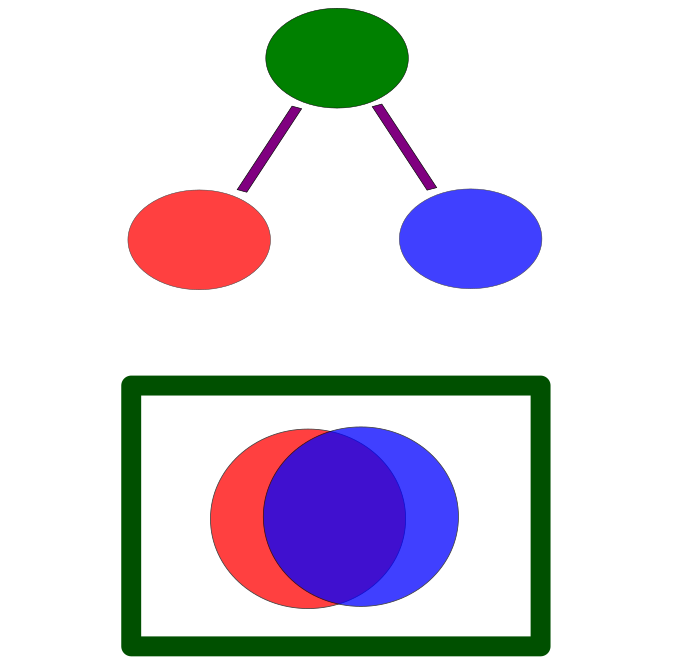
\includegraphics[width=\textwidth]{figures/RedundancyTrimmingOntogeny.png}
   	 	\caption{}
    \label{fig:simdiagram}
  \end{subfigure}
  %
  \begin{subfigure}[b]{0.3\textwidth}
    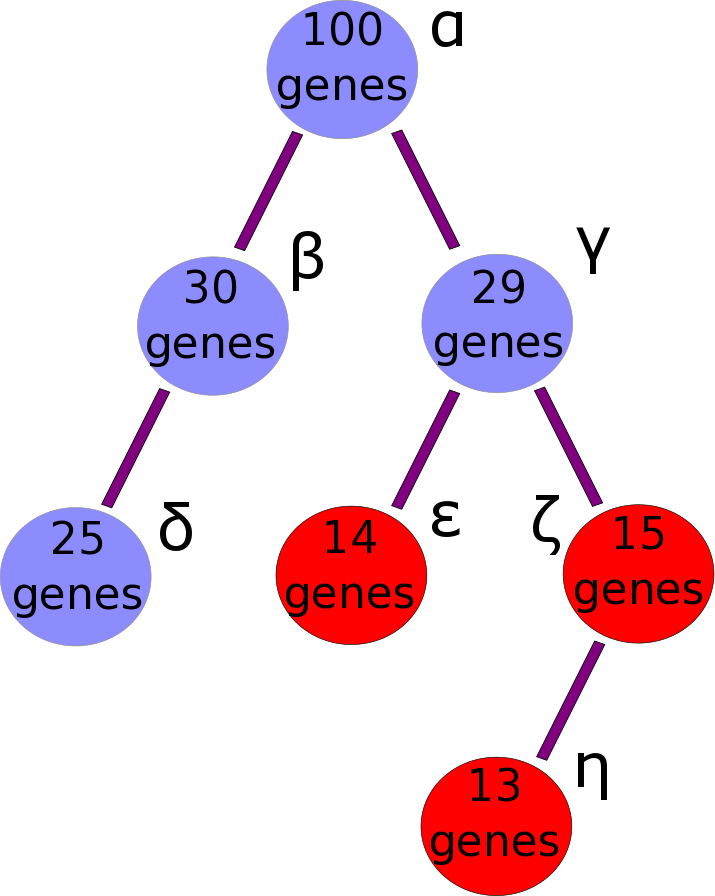
\includegraphics[width=\textwidth]{figures/FloorTrimmingOntogeny.png}
	      \caption{}
    \label{fig:trim_ends}
  \end{subfigure}
  \begin{subfigure}[b]{0.3\textwidth}
    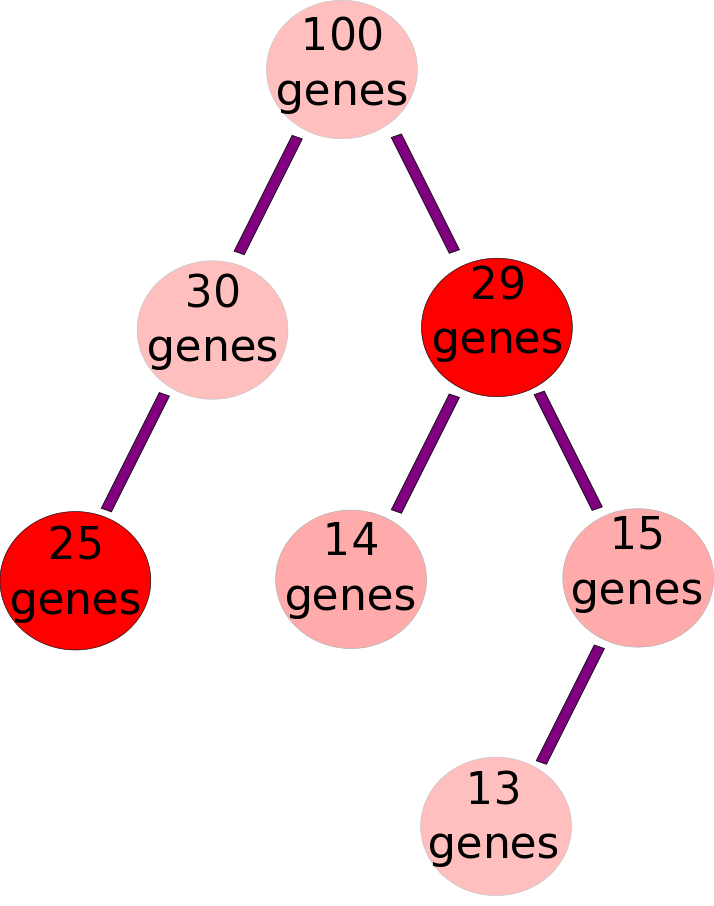
\includegraphics[width=\textwidth]{figures/CeilingTrimmingOntogeny.png}
    	\caption{}
    \label{fig:trim_roots}
  \end{subfigure}

  \captionsetup{width= 0.95\textwidth}
  \caption{
  	\csentence{Schematic representation of trimming filters for an acyclical ontology.}
    \csentence{\textbf{a)}} The parent node (green) contains at least as many annotations as the union of the two sisters. These two sisters share annotations extensively, as expressed by the overlap in the Venn diagram, so they qualify for removal. 	
	\csentence{\textbf{b)}} Nodes with less than a threshold number of genes are trimmed (red) and discarded from the dictionary. Here, the example threshold is 25 genes. Nodes $\epsilon, \zeta, \eta$, shown in red are removed.
	\csentence{\textbf{c)}} Parent nodes are removed recursively, starting from the root, if all their daughter nodes have more than the threshold number of annotations. Nodes in grey ($\epsilon, \zeta, \eta$) were removed in the previous step. Nodes $\alpha, \beta$ shown in red are trimmed because each one has a complete daughter set. Only nodes $\gamma$ and $\delta$ will be used to generate the static dictionary. 
  }
\end{figure}



%gui
\begin{figure}
	\centering
    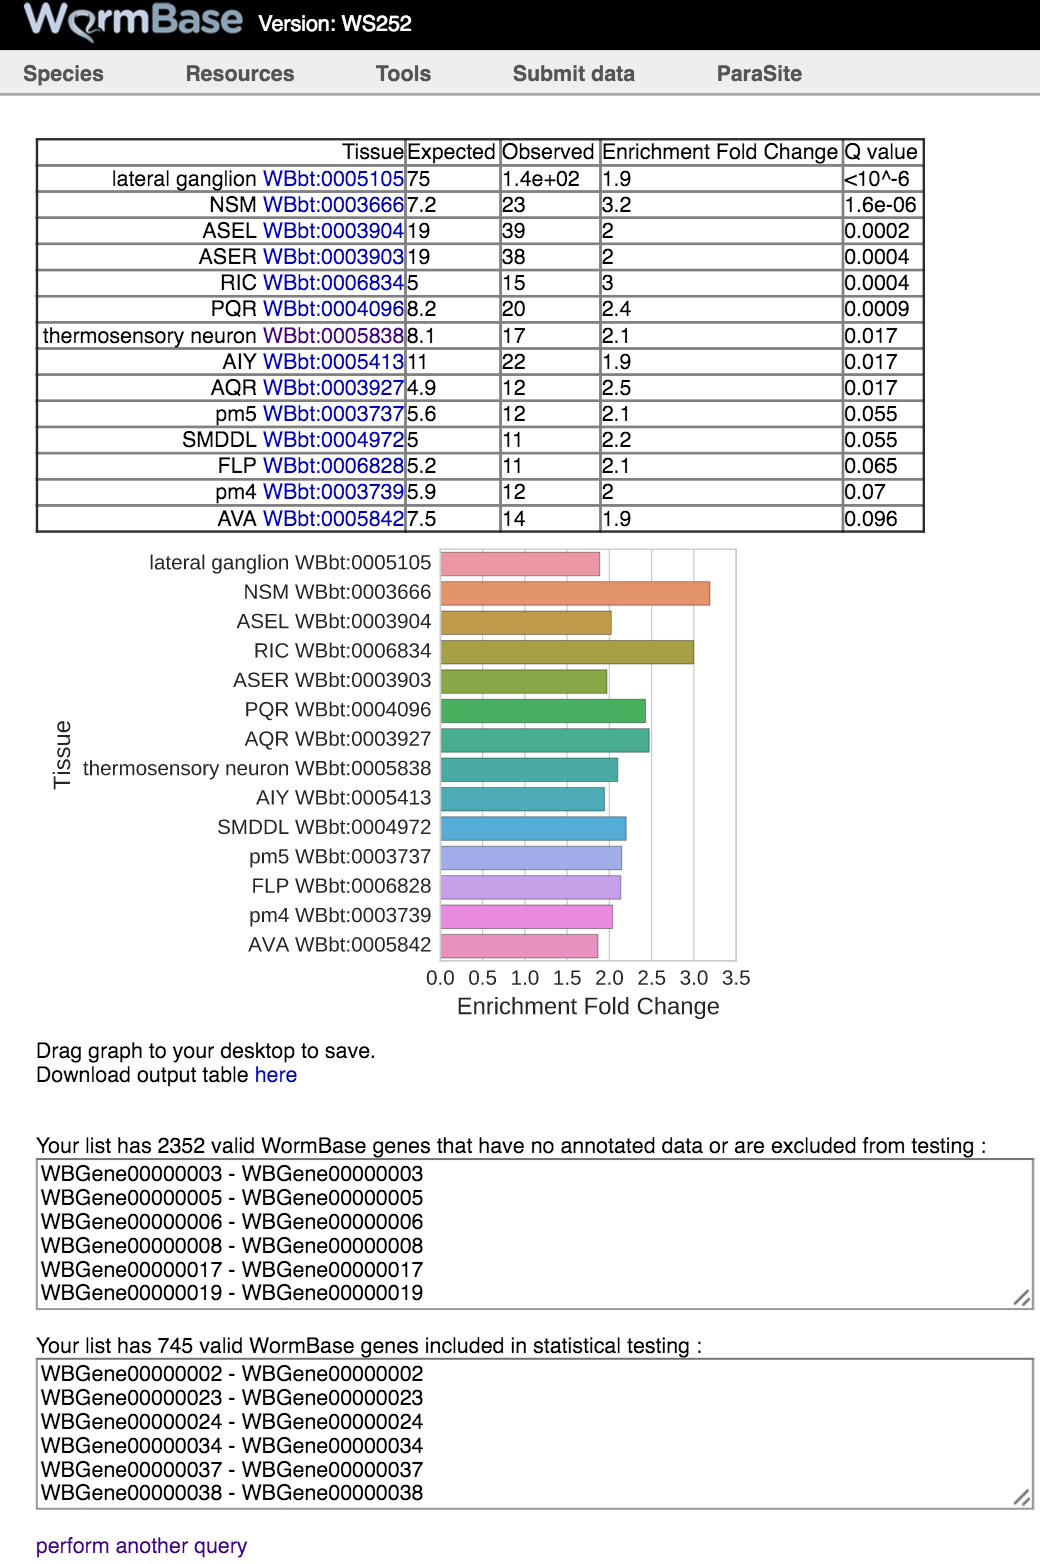
\includegraphics[width=0.95\textwidth]{figures/guiresults.png}
  	\captionsetup{width= 0.95\textwidth}
 	\caption{
	\csentence{Screenshot of results from the web GUI.} 
	After inputting a gene-list, the user is provided with the results. An HTML table is output with hyperlinks to the ontology terms. A publication-ready graph is provided below, which can be saved by  dragging to the desktop. The graph is colored for better visualization; color is not intended to convey information. The graph and the table show anatomy terms in  human-readable format, followed by their unique WBbt ID. Finally, lists  of the genes used and discarded for the analysis are also presented.
  }
  \label{fig:GUIresults}
\end{figure}


% workflow 
\begin{figure}
	\centering
	\includegraphics[width=0.95\textwidth]{figures/workflow.pdf}
	\captionsetup{width= 0.95\textwidth}
	\caption{
	\csentence{TEA Workflow.}
	The complete ontology is annotated continuously by WormBase curators. After each update, the ontology is processed to remove uninformative terms. The trimmed ontology is used for statistical testing. 
	Users can select a gene list and input it into our tool using our WormBase portal. The gene list is tested for enrichment using the trimmed ontology, and results are output in tabular and graphic formats for analysis. 
	}
	\label{fig:workflow}
\end{figure}


% statistical testing and validation Figures
%q plot
\begin{figure}[h!]
	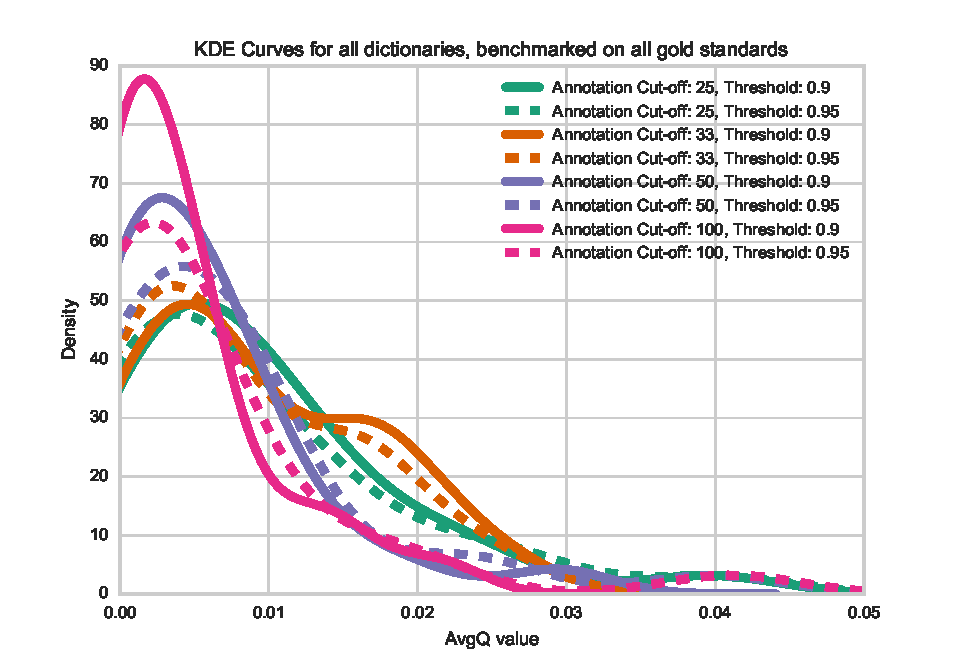
\includegraphics[width=\textwidth]{avgQKDE_method=any.pdf}
  \captionsetup{width= 0.95\textwidth}
  \caption{
  \csentence{Kernel density estimates for 30 gold standard datasets.}
      We ran TEA on 30 datasets we believed to be enriched in particular tissues and pooled all the results to observe the distribution of q-values. The mode of the distribution for dictionaries with annotation cut-offs of 100 and 50 genes are very similar; however, when the cut-off is lowered to 25 genes, the mode of the distribution shifts to the left, potentially signalling a decrease in measurement power.
	  }
	  \label{fig:qvals}
\end{figure}



%gaba
\begin{figure}
  \includegraphics[width=0.95\textwidth]{GABAcomparison3.pdf}
  \captionsetup{width= 0.95\textwidth}
  \caption{
  \csentence{Independently derived gene sets show similar results 	when tested with the same dictionary.}
  \textbf{Set 1)} GABAergic gene set from Watson~\cite{Watson2008a}.
  \textbf{Set 2)} GABAergic gene set from Spencer~\cite{Spencer2011}.
  Arrowheads highlight identical terms between both analyses. All terms refer to neurons or neuronal tissues and are GABA-associated. Dictionary with cutoff: 33; threshold: 0.95; method: `any'.
   }
  \label{fig:intragree}
\end{figure}


%results Figures - engelmann et al reanalysis
%labels are missing.
\begin{figure}[h!]
    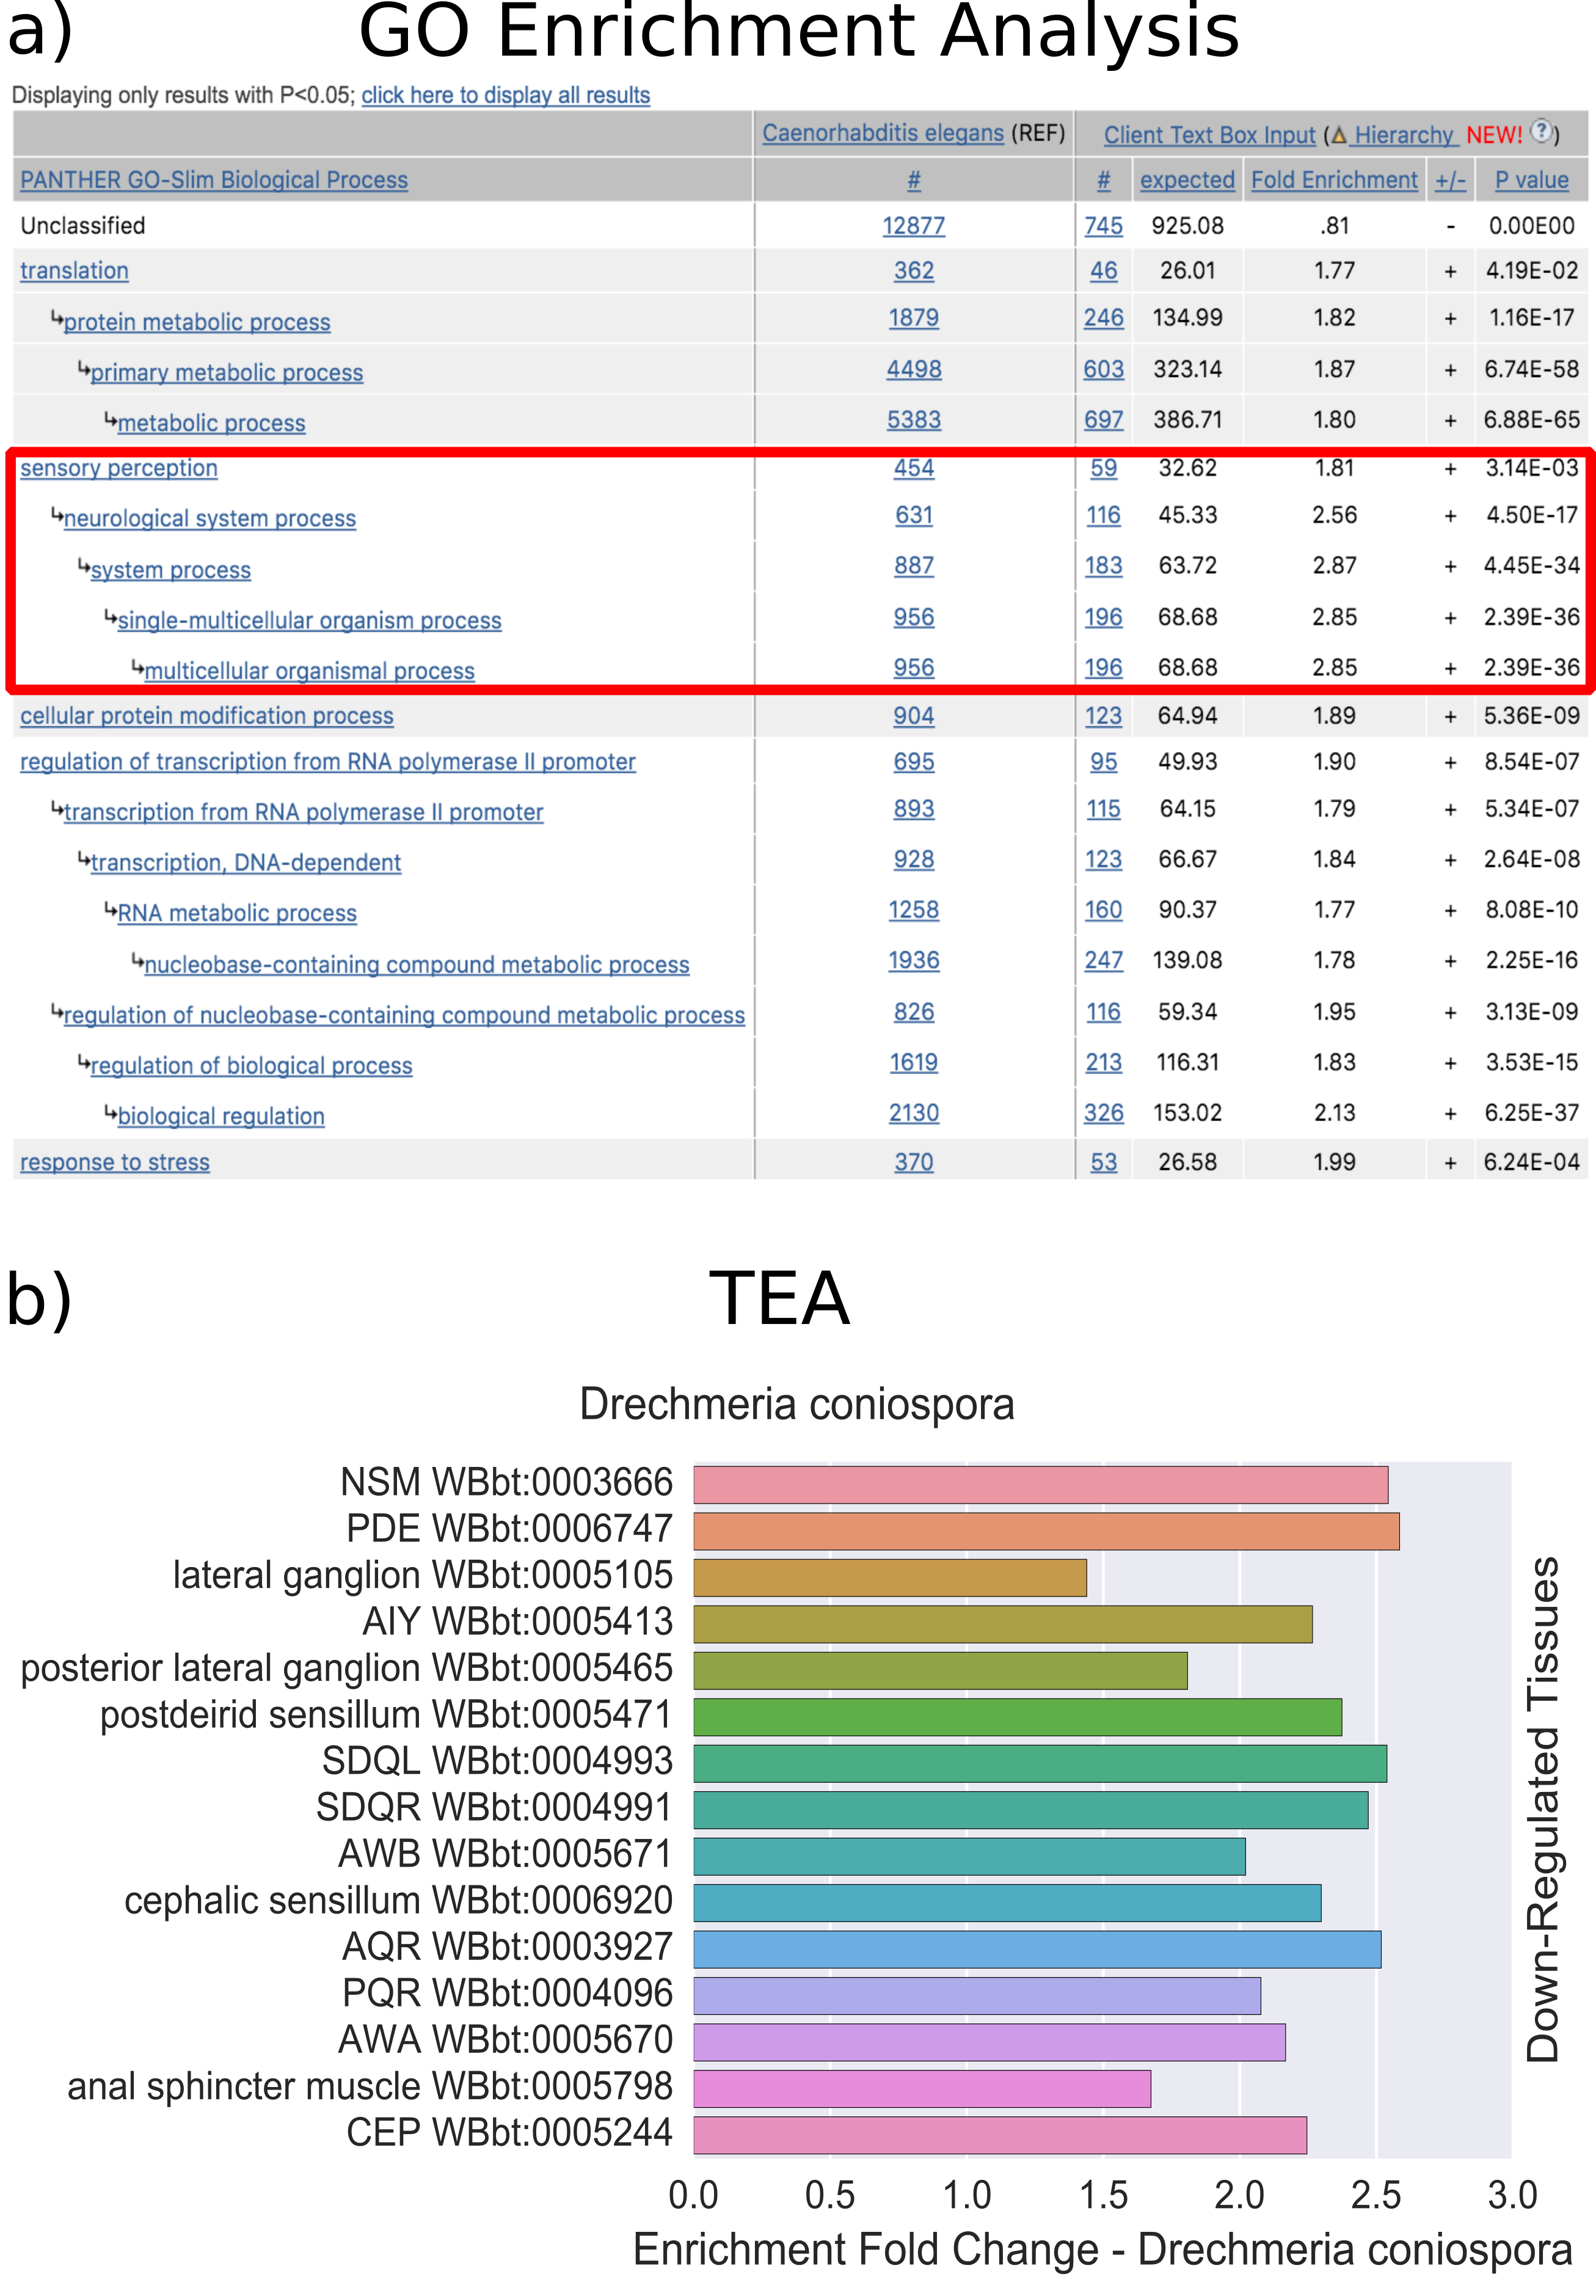
\includegraphics[width=0.95\textwidth]{figures/engelmann-GO-tea-comparison.png}
	\captionsetup{width= 0.95\textwidth}
  	\caption{
	\csentence{\emph{D.~coniospora} Gene Enrichment Analysis and Tissue Enrichment Analysis results.}
	We compared and contrasted the results from a gene enrichment analysis program, pantherDB, with TEA by analyzing genes that were significantly down-regulated when \emph{C.~elegans} was exposed to \emph{D.~coniospora} in a previously published dataset by Engelmann \emph{et al}~\cite{Engelmann2011} with both tools. 
	\textbf{a)} pantherDB screenshot of results, sorted by p-value. Only top hits shown.
	\textbf{b)} TEA results, sorted by q-value (lowest on top) and fold-change. 
	Both pantherDB and TEA identify terms associated with neurons (red square). The two analyses provide complementary, not redundant, information.
	}
	\label{fig:Dcon}
\end{figure}


%%%%%%%%%%%%%%%%%%%%%%%%%%%%%%%%%%%
%%                               %%
%% Tables                        %%
%%                               %%
%%%%%%%%%%%%%%%%%%%%%%%%%%%%%%%%%%%

%% Use of \listoftables is discouraged.
%%
\section*{Tables}

\begin{table}[h!]
	\caption{
	Parameter specifications and number of tissues for all dictionaries. The `Method' column refers to the trimming criterion for the similarity metric. We used two such criteria, `any' and `avg'.`any': For a given sister set, if any sister had a similarity exceeding the corresponding threshold, all sisters were removed from the final dictionary. `avg': For a given sister set, if the average similarity across all the sisters in the set was greater than the corresponding threshold, all sisters were removed from the final dictionary.
	}
	\csvreader[tabular= c | c | c | c,
	table head= {\textbf{Annotation Cutoff}} & {\textbf{Similarity Threshold}} & {\textbf{Method}} & {\textbf{No. Of Terms in Dictionary}}\\\hline,
	late after line= \\,
	late after last line= \\\hline
	]
	{figures/TissueNumbers.csv}{}
	{\csvcoli & \csvcolii & \csvcoliii & \csvcoliv}	
	
	% \csvautotabular{figures/TissueNumbers.csv}
	\label{tab:DictionarySpecs}
\end{table}

\begin{table}[h!]
	\caption{
	Comparison of results for a neuronal-enriched gene set from Watson~\cite{Watson2008a}. We ran the same genelist on a dictionary with a minimum annotation cutoff of 50, similarity threshold of 0.95 and similarity method `any' versus another with a minimum annotation cutoff of 33, similarity threshold of 0.95 and similarity method `any'. In the table, columns are labeled with their significance value (Q-value) or enrichment fold change followed by a hyphen and a number which indicates which the cutoff for the dictionary that was used for testing. Not all tissues are present in either dictionary. Hyphens denote not-applicable values, which occurs when a particular tissue is not present in both dictionaries. Full table is available on github.
	}
	
	\begin{adjustbox}{width=1\textwidth}
		\centering
		% \csvreader{figures/dict-comparison-50-33.csv}
		\csvreader[tabular={ r | c | c | c | c},
	    table head ={\textbf{Tissue}} & {\textbf{Q-value-33}} & {\textbf{Q-value-50}} & {\textbf{Enrichment-33}} & {\textbf{Enrichment-50}}\\\hline,
	    late after line= \\,
		late after last line=\\\hline
		]%
		{figures/dict-comparison-50-33.csv}{}	
		{\csvcoli & \csvcolii & \csvcoliii & \csvcoliv & \csvcolv}	
		\label{tab:interagree}
	\end{adjustbox}
\end{table}

%%%%%%%%%%%%%%%%%%%%%%%%%%%%%%%%%%%
%%                               %%
%% Additional Files              %%
%%                               %%
%%%%%%%%%%%%%%%%%%%%%%%%%%%%%%%%%%%

\section*{Additional Files}
  \subsection*{Additional file 1 --- IPython Notebook}
    Tutorial for users interested in using our software within a python script


\end{backmatter}
\end{document}